%%
%% This is file `sample-manuscript.tex',
%% generated with the docstrip utility.
%%
%% The original source files were:
%%
%% samples.dtx  (with options: `manuscript')
%% 
%% IMPORTANT NOTICE:
%% 
%% For the copyright see the source file.
%% 
%% Any modified versions of this file must be renamed
%% with new filenames distinct from sample-manuscript.tex.
%% 
%% For distribution of the original source see the terms
%% for copying and modification in the file samples.dtx.
%% 
%% This generated file may be distributed as long as the
%% original source files, as listed above, are part of the
%% same distribution. (The sources need not necessarily be
%% in the same archive or directory.)
%%
%% Commands for TeXCount
%TC:macro \cite [option:text,text]
%TC:macro \citep [option:text,text]
%TC:macro \citet [option:text,text]
%TC:envir table 0 1
%TC:envir table* 0 1
%TC:envir tabular [ignore] word
%TC:envir displaymath 0 word
%TC:envir math 0 word
%TC:envir comment 0 0
%%
%%
%% The first command in your LaTeX source must be the \documentclass command.
%%%% Small single column format, used for CIE, CSUR, DTRAP, JACM, JDIQ, JEA, JERIC, JETC, PACMCGIT, TAAS, TACCESS, TACO, TALG, TALLIP (formerly TALIP), TCPS, TDSCI, TEAC, TECS, TELO, THRI, TIIS, TIOT, TISSEC, TIST, TKDD, TMIS, TOCE, TOCHI, TOCL, TOCS, TOCT, TODAES, TODS, TOIS, TOIT, TOMACS, TOMM (formerly TOMCCAP), TOMPECS, TOMS, TOPC, TOPLAS, TOPS, TOS, TOSEM, TOSN, TQC, TRETS, TSAS, TSC, TSLP, TWEB.
% \documentclass[acmsmall]{acmart}

%%%% Large single column format, used for IMWUT, JOCCH, PACMPL, POMACS, TAP, PACMHCI
% \documentclass[acmlarge,screen]{acmart}

%%%% Large double column format, used for TOG
% \documentclass[acmtog, authorversion]{acmart}

%%%% Generic manuscript mode, required for submission
%%%% and peer review
\documentclass[manuscript,screen,review]{acmart}

%% 追加
\usepackage{bm}
\newcommand\figref[1]{\textbf{Figure~\ref{fig:#1}}}
\newcommand\tabref[1]{\textbf{Table~\ref{tab:#1}}}
\usepackage{url}
\usepackage{color}
\usepackage{multirow}
\usepackage{diagbox}
\usepackage[subrefformat=parens]{subcaption}
\captionsetup{compatibility=false}
%% ここまで

%% Fonts used in the template cannot be substituted; margin 
%% adjustments are not allowed.
%%
%% \BibTeX command to typeset BibTeX logo in the docs
\AtBeginDocument{%
  \providecommand\BibTeX{{%
    \normalfont B\kern-0.5em{\scshape i\kern-0.25em b}\kern-0.8em\TeX}}}

%% Rights management information.  This information is sent to you
%% when you complete the rights form.  These commands have SAMPLE
%% values in them; it is your responsibility as an author to replace
%% the commands and values with those provided to you when you
%% complete the rights form.
\setcopyright{acmcopyright}
\copyrightyear{2018}
\acmYear{2018}
\acmDOI{XXXXXXX.XXXXXXX}

%% These commands are for a PROCEEDINGS abstract or paper.
\acmConference[Conference acronym 'XX]{Make sure to enter the correct
  conference title from your rights confirmation emai}{June 03--05,
  2018}{Woodstock, NY}
%
%  Uncomment \acmBooktitle if th title of the proceedings is different
%  from ``Proceedings of ...''!
%
\acmBooktitle{Woodstock '18: ACM Symposium on Neural Gaze Detection,
 June 03--05, 2018, Woodstock, NY} 
\acmPrice{15.00}
\acmISBN{978-1-4503-XXXX-X/18/06}


%%
%% Submission ID.
%% Use this when submitting an article to a sponsored event. You'll
%% receive a unique submission ID from the organizers
%% of the event, and this ID should be used as the parameter to this command.
%%\acmSubmissionID{123-A56-BU3}

%%
%% For managing citations, it is recommended to use bibliography
%% files in BibTeX format.
%%
%% You can then either use BibTeX with the ACM-Reference-Format style,
%% or BibLaTeX with the acmnumeric or acmauthoryear sytles, that include
%% support for advanced citation of software artefact from the
%% biblatex-software package, also separately available on CTAN.
%%
%% Look at the sample-*-biblatex.tex files for templates showcasing
%% the biblatex styles.
%%

%%
%% The majority of ACM publications use numbered citations and
%% references.  The command \citestyle{authoryear} switches to the
%% "author year" style.
%%
%% If you are preparing content for an event
%% sponsored by ACM SIGGRAPH, you must use the "author year" style of
%% citations and references.
%% Uncommenting
%% the next command will enable that style.
%%\citestyle{acmauthoryear}

%%
%% end of the preamble, start of the body of the document source.
\begin{document}

%%
%% The "title" command has an optional parameter,
%% allowing the author to define a "short title" to be used in page headers.
\title{Smart Faucet: Overflow Detection by Sensing Water Drop Sound}

%%
%% The "author" command and its associated commands are used to define
%% the authors and their affiliations.
%% Of note is the shared affiliation of the first two authors, and the
%% "authornote" and "authornotemark" commands
%% used to denote shared contribution to the research.
\author{Atsuhiro Fujii}
\email{atsuhiro.fujii@iis.ise.ritsumei.ac.jp}
\affiliation{%
  \institution{Ritsumeikan University}
  \city{Shiga}
  \country{Japan}
}

\author{Kazuya Murao}
\email{murao@cs.ritsumei.ac.jp}
\affiliation{%
  \institution{Ritsumeikan University}
  \city{Shiga}
  \country{Japan}
}

%%
%% By default, the full list of authors will be used in the page
%% headers. Often, this list is too long, and will overlap
%% other information printed in the page headers. This command allows
%% the author to define a more concise list
%% of authors' names for this purpose.
\renewcommand{\shortauthors}{Fujii and Murao}

%%
%% The abstract is a short summary of the work to be presented in the
%% article.
\begin{abstract}
  There are many situations in daily life where liquids are poured into containers. When pouring a beverage or other liquid into an opaque, narrow-mouthed container such as a ceramic sake bottle or aluminum can, it is difficult to accurately ascertain the level of water in the container visually, and the liquid may overflow. Therefore, we need a method other than visual inspection for determining the water level in a container. One option would be using a liquid level sensor, but this is complicated because a device would need to be attached to each container. We therefore propose a method that senses the sound generated when pouring liquid into the container. As this method estimates the water level inside a container by acquiring the pouring sound from outside the container, it is highly versatile in that it does not require the installation of a device for each container. The results of evaluation experiments showed that for the estimation of water level from 0\% to 100\% in increments of 10\%, the estimation accuracy averaged 0.462 and 0.308 for bottle-dependent and bottle-independent estimation models, respectively. As for the model that estimates whether the water level is above 90\% or not, the average estimation accuracy of 0.744 was achieved, even bottle-independent estimation model was used. These results indicate that, while the estimation accuracy needs to be improved in the case of water-level estimation, the proposed method has the potential to be used in real environments for application to overflow detection. In future work, we will implement a faucet-mounted device that incorporates a function to stop water pouring just before it fills up.
\end{abstract}

%%
%% The code below is generated by the tool at http://dl.acm.org/ccs.cfm.
%% Please copy and paste the code instead of the example below.
%%
\begin{CCSXML}
<ccs2012>
 <concept>
  <concept_id>10010520.10010553.10010562</concept_id>
  <concept_desc>Computer systems organization~Embedded systems</concept_desc>
  <concept_significance>500</concept_significance>
 </concept>
 <concept>
  <concept_id>10010520.10010575.10010755</concept_id>
  <concept_desc>Computer systems organization~Redundancy</concept_desc>
  <concept_significance>300</concept_significance>
 </concept>
 <concept>
  <concept_id>10010520.10010553.10010554</concept_id>
  <concept_desc>Computer systems organization~Robotics</concept_desc>
  <concept_significance>100</concept_significance>
 </concept>
 <concept>
  <concept_id>10003033.10003083.10003095</concept_id>
  <concept_desc>Networks~Network reliability</concept_desc>
  <concept_significance>100</concept_significance>
 </concept>
</ccs2012>
\end{CCSXML}

\ccsdesc[500]{Computer systems organization~Embedded systems}
\ccsdesc[300]{Computer systems organization~Redundancy}
\ccsdesc{Computer systems organization~Robotics}
\ccsdesc[100]{Networks~Network reliability}

%%
%% Keywords. The author(s) should pick words that accurately describe
%% the work being presented. Separate the keywords with commas.
\keywords{smart device, smart home, ubiquitous computing, faucet, water level, acoustic sensing, acoustic recognition}

%% A "teaser" image appears between the author and affiliation
%% information and the body of the document, and typically spans the
%% page.
% \begin{teaserfigure}
%   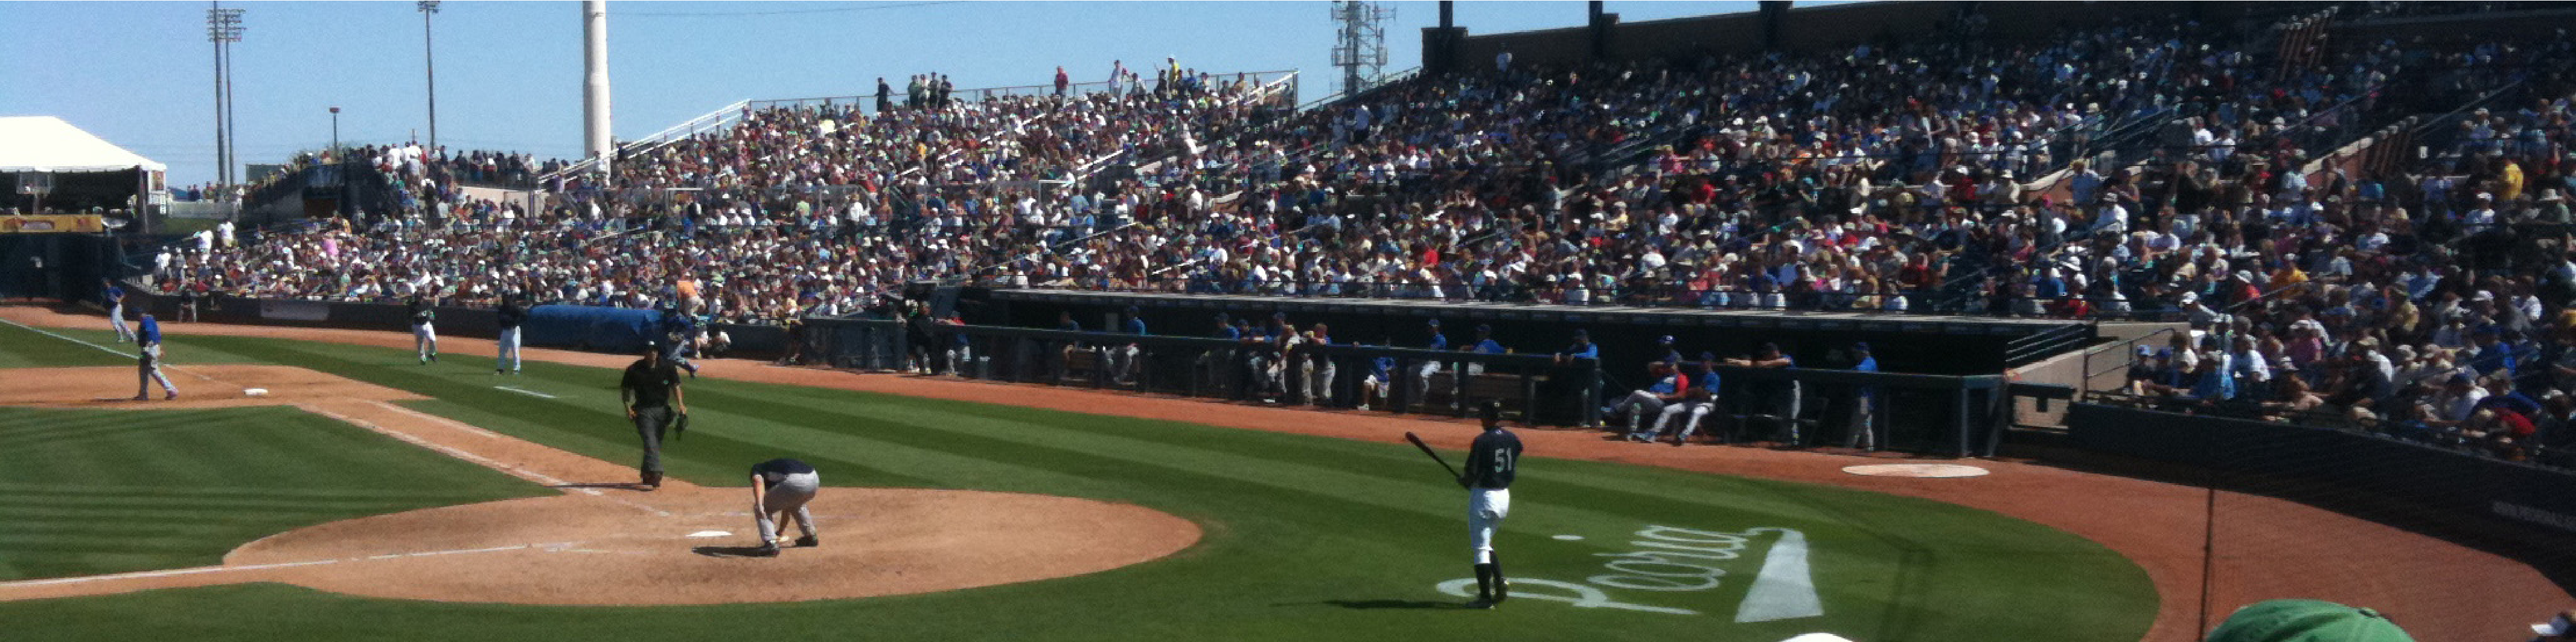
\includegraphics[width=\textwidth]{sampleteaser}
%   \caption{Seattle Mariners at Spring Training, 2010.}
%   \Description{Enjoying the baseball game from the third-base
%   seats. Ichiro Suzuki preparing to bat.}
%   \label{fig:teaser}
% \end{teaserfigure}

\received{20 February 2007}
\received[revised]{12 March 2009}
\received[accepted]{5 June 2009}

%%
%% This command processes the author and affiliation and title
%% information and builds the first part of the formatted document.
\maketitle

% 1
\section{Introduction}
There are many situations in daily life where liquids are poured into containers. When a liquid is poured into a transparent container such as a glass cup, it is unlikely for the liquid to overflow because the water level inside the container can be ascertained. However, when pouring into an opaque, narrow-mouthed container such as a ceramic sake bottle or aluminum can, it is difficult to correctly gauge the level of water in the container by visual inspection, and overflow may occur. Water and other beverages can be wiped up fairly easily if they overflow, but highly hazardous liquids such as paint and kerosene are more difficult and could lead to an accident. We therefore believe it is necessary to determine the water level in a container using a method other than visual inspection. In this vein, Ren et al. \cite{LiquidSense} proposed LiquidSense, a liquid level sensing system that utilizes an existing home Wi-Fi network and low-cost transducers attached to the surface of the container to detect resonances inside the container and identify the liquid level. In addition, small liquid level sensors are commercially available for microcontrollers \footnote{\url{http://sfe.io/p10221}}. The downside of these methods and sensors is that they require a device to be attached to each container.\par

One way of obtaining the water level without modifying the container is to use an ultrasonic sensor to estimate the water volume based on the distance to the water surface \cite{smart_faucet1}. However, when this type of sensor is installed on a faucet, estimation is difficult because the distance from the faucet to the container is not constant when the container is held in the hand. Another possible method is to install a camera on the faucet and use image recognition to estimate the water volume, but the estimation accuracy may be degraded in dark areas. Since there are also faucets that discharge water at an angle, estimation methods using ultrasonic sensors or cameras may not be able to obtain the correct distance when pouring water into containers with a small caliber.\par

In this study, we propose a method to estimate the water level in a container by recording the sound of liquid pouring into it. Since our method estimates the water level inside a container by acquiring the sound of water pouring outside the container, it is highly versatile in the sense that there is no need to install a device for each container. Moreover, since the estimation method utilizes sound features, lighting conditions have no effect on the accuracy. It is also unlikely to be affected by changes in the faucet or the caliber of the container. In this paper, the sound generated when pouring a liquid into a container is referred to as ``pouring sound''. The water level can be estimated as long as this sound is generated when the liquid is poured into the container, even for liquids other than water. The proposed method uses only a microphone as a sensor, so it can be installed in various environments. For example, it could be implemented as a smart faucet that stops pouring water just before it overflows, or as a smartphone application that displays the estimated water level on the screen. Gasoline refueling nozzles are equipped with an automatic refueling stop device that based on the Venturi effect, but the device does not work when refueling small fuel tanks such as those in motorcycles, and must be manually adjusted to prevent overflow. Moreover, the small caliber of the fueling port makes it difficult to visually check the content of the fuel tank. Implementation as a smartphone app is effective in such situations. The user simply holds the smartphone next to the fuel tank when refueling, and the app estimates the amount of fuel in the tank and notifies the user before it overflows. We feel that preventing overflows will reduce the wasteful use of resources and help protect the environment. This paper investigates the feasibility of estimating water volume using the pouring sound as a preliminary step for implementation in various devices.\par

Section \ref{sec:related} introduces related works, section \ref{sec:method} describes the details of the proposed method, section \ref{sec:evaluation} presents our evaluation, and section \ref{sec:future_work} discusses future plans. We conclude in section \ref{sec:conclution} with a brief summary.



% 2
\section{Related Work}
\label{sec:related}
This section introduces innovations in smart homes, recognition based on sound, and estimation of water volume.

% 2.1
\subsection{Innovations in Smart Homes}
Xu et al. \cite{smart_home1} proposed a smart coffee roaster that can monitor bean temperature and carbon monoxide content from a smartphone or tablet application.
Hirai et al. \cite{smart_home2} proposed a ceiling-based display system that can simultaneously display a variety of information.
Hossain et al. \cite{smart_home3} proposed a sensor-based smart bathtub system that improves safety and saves water by recognizing human activity in the bathtub.
There are also several studies on smart refrigerators \cite{smart_refrigerator1, smart_refrigerator2, smart_refrigerator3, smart_refrigerator4}. \par

Chiu et al. \cite{PlayfulBottle} proposed a system in which a cell phone is attached to a daily-use mug to motivate office workers to drink a healthy amount of water.
Tommy et al. \cite{SmartBottle} proposed a smart bottle that measures water consumption in real time and notifies the user through an Android smartphone app, where the bottle and smartphone are connected via seamless Bluetooth.
Kaner et al. \cite{GROW} developed Grow, a prototype smart bottle designed to encourage users to drink water regularly. An integrated liquid level sensor records daily water intake, and the surface of the bottle is used as an ambient display to provide feedback.\par

Al-Yemni et al. \cite{smart_faucet2} proposed a smart faucet that dispenses temperature-controlled water calibrated to the user’s body temperature. The device is implemented with Arduino Uno and features a temperature sensor and two valves for hot and cold water, with the idea of reducing the amount of water wasted during water temperature control. It can be put to use simply by replacing the faucet, even in older facilities.
Sawidin et al. \cite{smart_faucet3} proposed a smart home control system utilizing Arduino Uno that controls the switching on/off of lights, opening and closing of house doors and garages, and opening and closing of faucets from an Android smartphone.
These studies are similar to ours in that they involve smart bottles and faucets, but none have focused on estimating water volume.


% 2.2
\subsection{Recognition Based on Sound}
Kato et al. \cite{sound_sensing1} proposed a hand state recognition method based on active acoustic sensing of the wrist area to achieve an intuitive user interface. Their method utilizes the power spectral density of bone-conducted sound as a feature and performs state recognition with a support vector machine.
Li et al. \cite{Auto++} proposed a system that detects approaching vehicles by utilizing the acoustic signals acquired from a microphone built into the user's smartphone. Their system not only detects the presence of a vehicle but also estimates the direction in which the vehicle is traveling as well as the number of vehicles around the user.
Chauhan et al. \cite{BreathPrint} proposed a biometric authentication system based on breath sounds. The system acquires sound features by having the user hold the microphone of a smartphone or other device close to his or her nose and perform a breathing gesture, and then authenticates the user on the basis of those features.
Shih et al. \cite{Breeze} proposed a mobile application utilizing a smartphone microphone to continuously detect the state of breathing and perform breathing training.
Mujibiya et al. \cite{sound_sensing2} proposed a method that recognizes touch and gesture on the body by measuring ultrasonic signals generated on one part of the body on another part.
Schneegass et al. \cite{SkullConduct} proposed a personal authentication method based on individual differences in bone-conduction sounds in the skull. Their evaluation experiments showed that the method achieved the accuracy of 97.0\% for personal identification and the equal error rate of 6.9\% for personal authentication.


% 2.3
\subsection{Estimation of Water Volume}
Fan et al. \cite{SoQr} proposed SoQr, a sensor consisting of a speaker and a microphone that attaches to the outer surface of everyday items to estimate the amount of liquid contained inside. The sensor outputs a short sinusoidal probe sound to the container, the microphone records the impulse response, and a support vector machine then estimates the amount of the liquid. The results of 10-fold cross-validation using 19 common household products revealed a mean F-value greater than 0.96.
This method is similar to ours in that both are for estimating water volume, but our method differs in that it does not require the user to attach a device to the container.



% 3
\section{Proposed Method}
\label{sec:method}
This section describes the details of the proposed method.

% 3.1
\subsection{Overview}
The process flow of the proposed system is shown in \figref{method}. When the valve is manually opened and water injection starts, the system is activated and acquires 0.2 seconds of sound data from the microphone mounted on the device. Next, the feature extraction is performed, and the obtained features are fed into the estimation model. Finally, the water level $W$ output from the estimation model is compared with the threshold value $T_{level}$, and the valve is controlled in accordance with the comparison result. When $W<=T_{level}$, the series of processes from sound data acquisition is repeated with the valve open. When $W>T_{level}$, the valve is closed, water injection is stopped, and the system is terminated. The system is also terminated when the valve is manually closed.

\begin{figure}[!t]
  \centering
  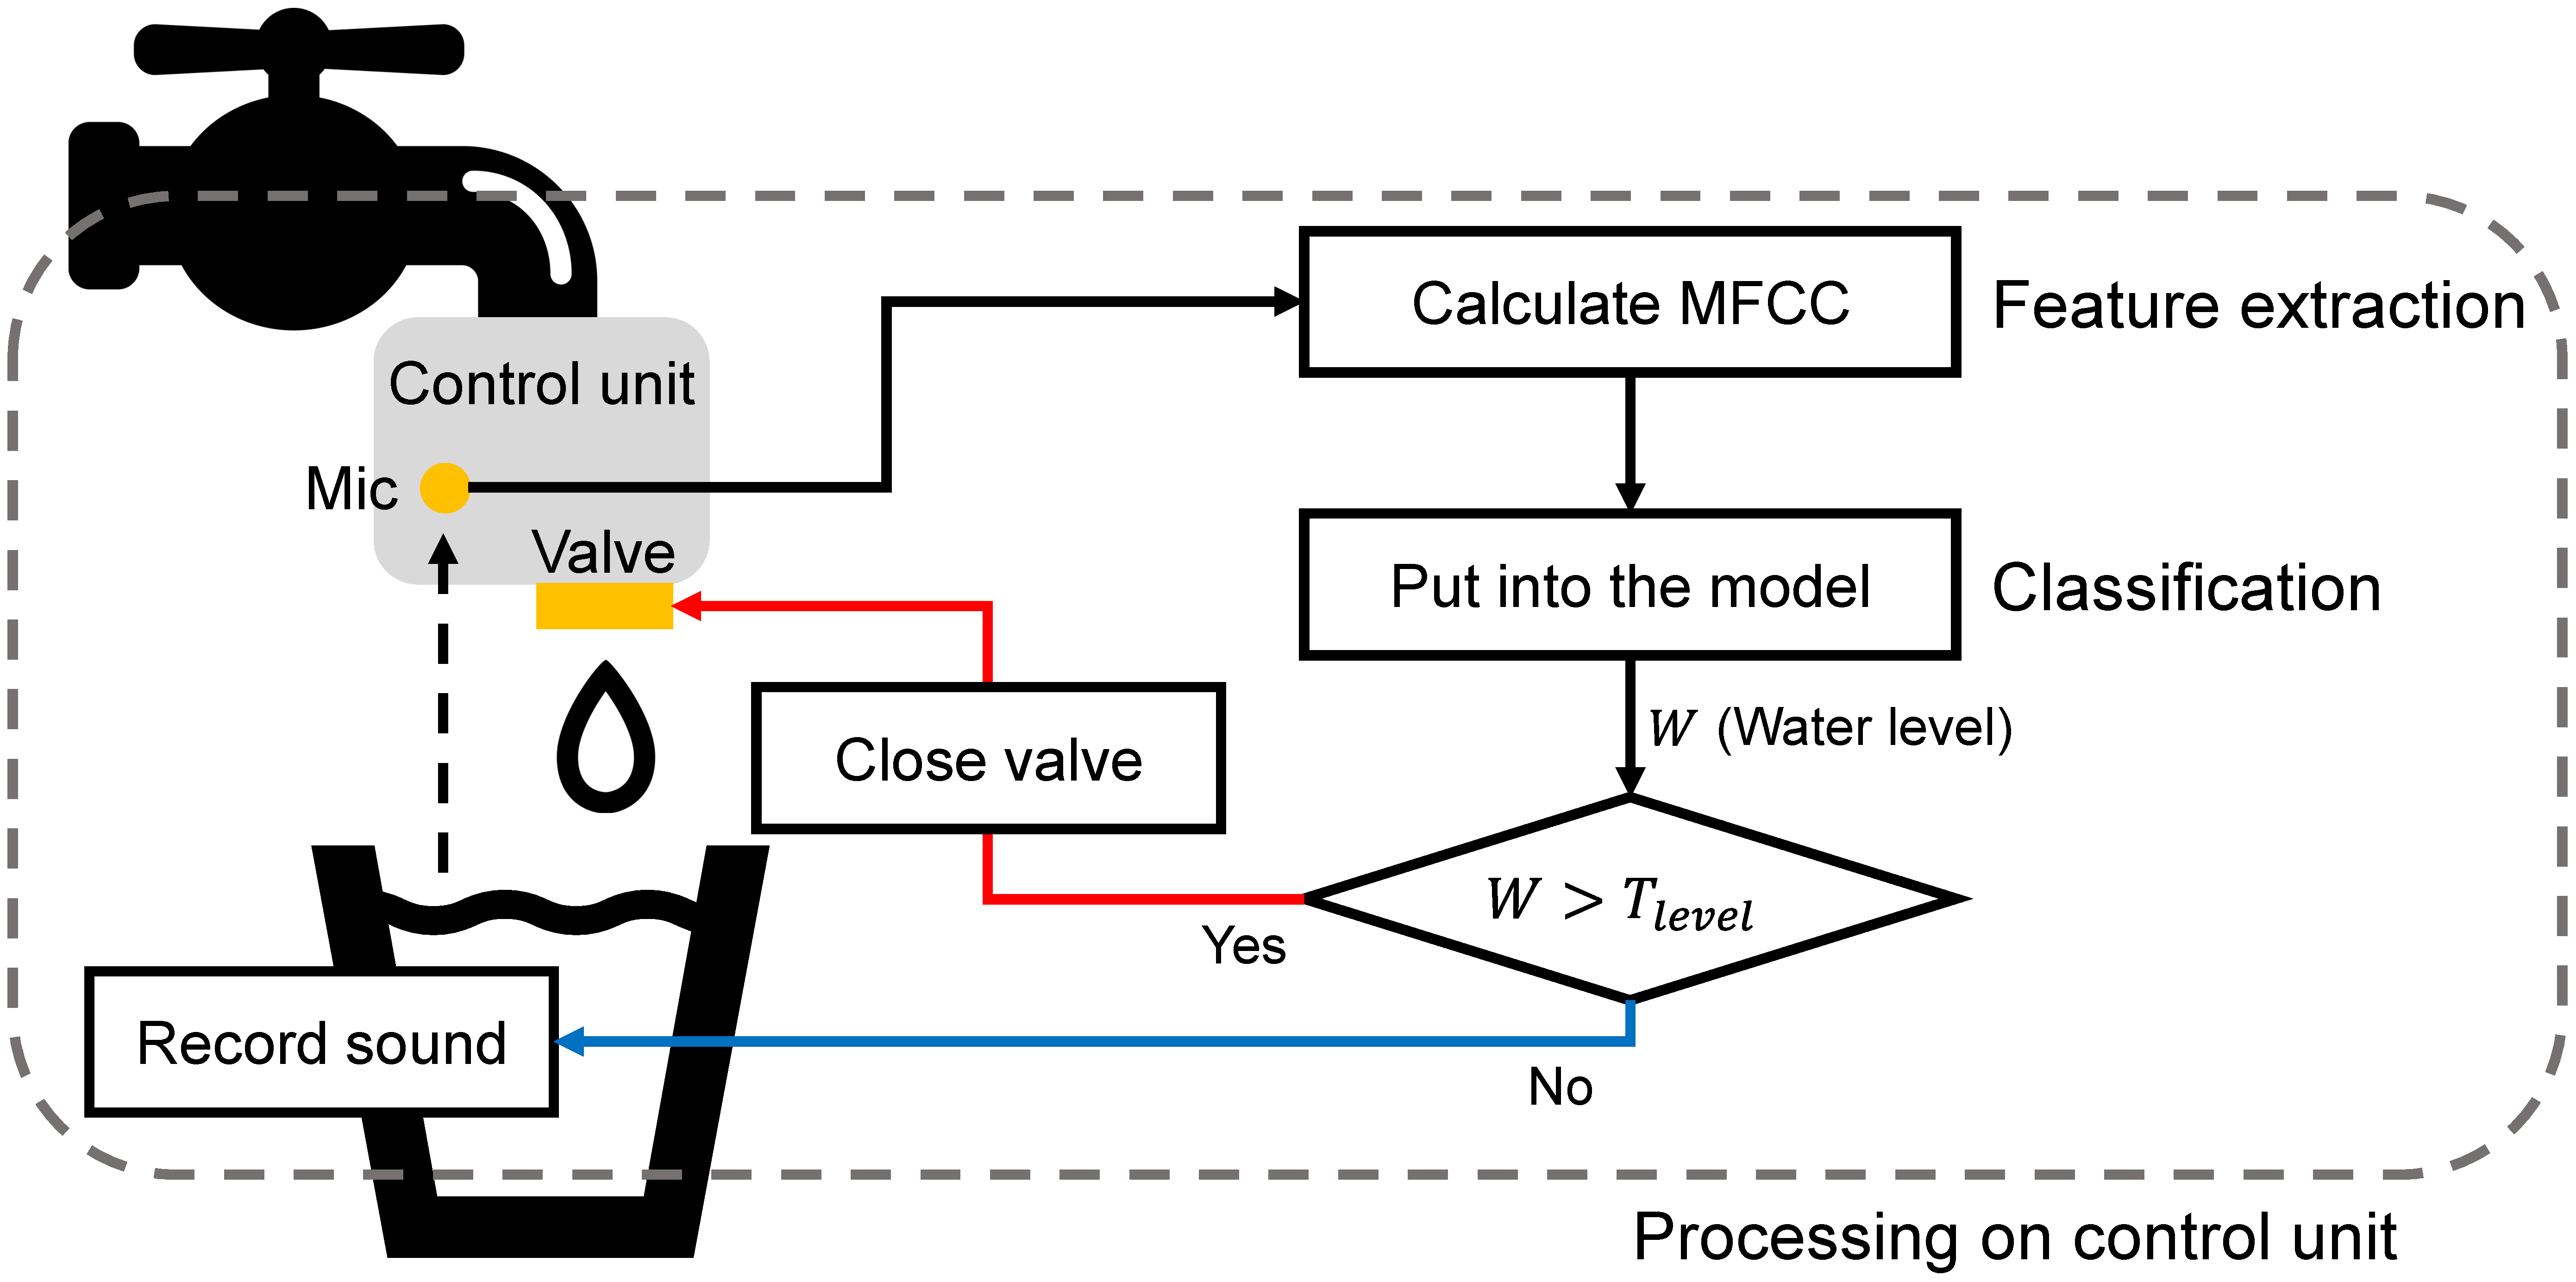
\includegraphics[width=0.8\linewidth]{figures/method.eps}
  \caption{Process flow of proposed system.}
  \label{fig:method}
\end{figure}


% 3.2
\subsection{Feature extraction}
The features are time-averaged Mel-frequency cepstral coefficients (MFCCs), which are commonly used in speech recognition. \texttt{librosa.feature.mfcc}\footnote{\url{https://librosa.org/doc/main/generated/librosa.feature.mfcc.html}} of LibROSA\footnote{\url{https://librosa.org}}, a Python acoustic signal processing library, was used to calculate MFCC. The argument $n\_mfcc$ to specify the number of MFCC dimensions is set to 61. After removing the first dimension data representing the orthogonal components of the data from the calculated MFCC, a time average is computed to extract features that are 1-dimensional and have a length of 60.


% 3.3
\subsection{Model}
The estimation model consists of three convolution layers, a ReLU function, a pooling layer, and a linear layer, as shown in \figref{model}. The values output from the linear layer are converted into probabilities of occurrence through the softmax function, and the label with the largest probability is selected in the activation layer. If there are multiple maximum probabilities, the label with the smallest index is adopted. The estimation model was implemented using PyTorch\footnote{\url{https://pytorch.org}}, with CrossEntropyLoss\footnote{\url{https://pytorch.org/docs/stable/generated/torch.nn.CrossEntropyLoss.html}} as the loss function and Adam\footnote{\url{https://pytorch.org/docs/stable/generated/torch.optim.Adam.html}} as the optimizer. The parameter $lr$ used in Adam was set to 0.0002. The kernel size used in Conv1d and MaxPool1d was set to be 3. The values output from the linear layer are used directly for training during the training phase, as CrossEntropyLoss incorporates a softmax function.

\begin{figure}[!t]
  \centering
  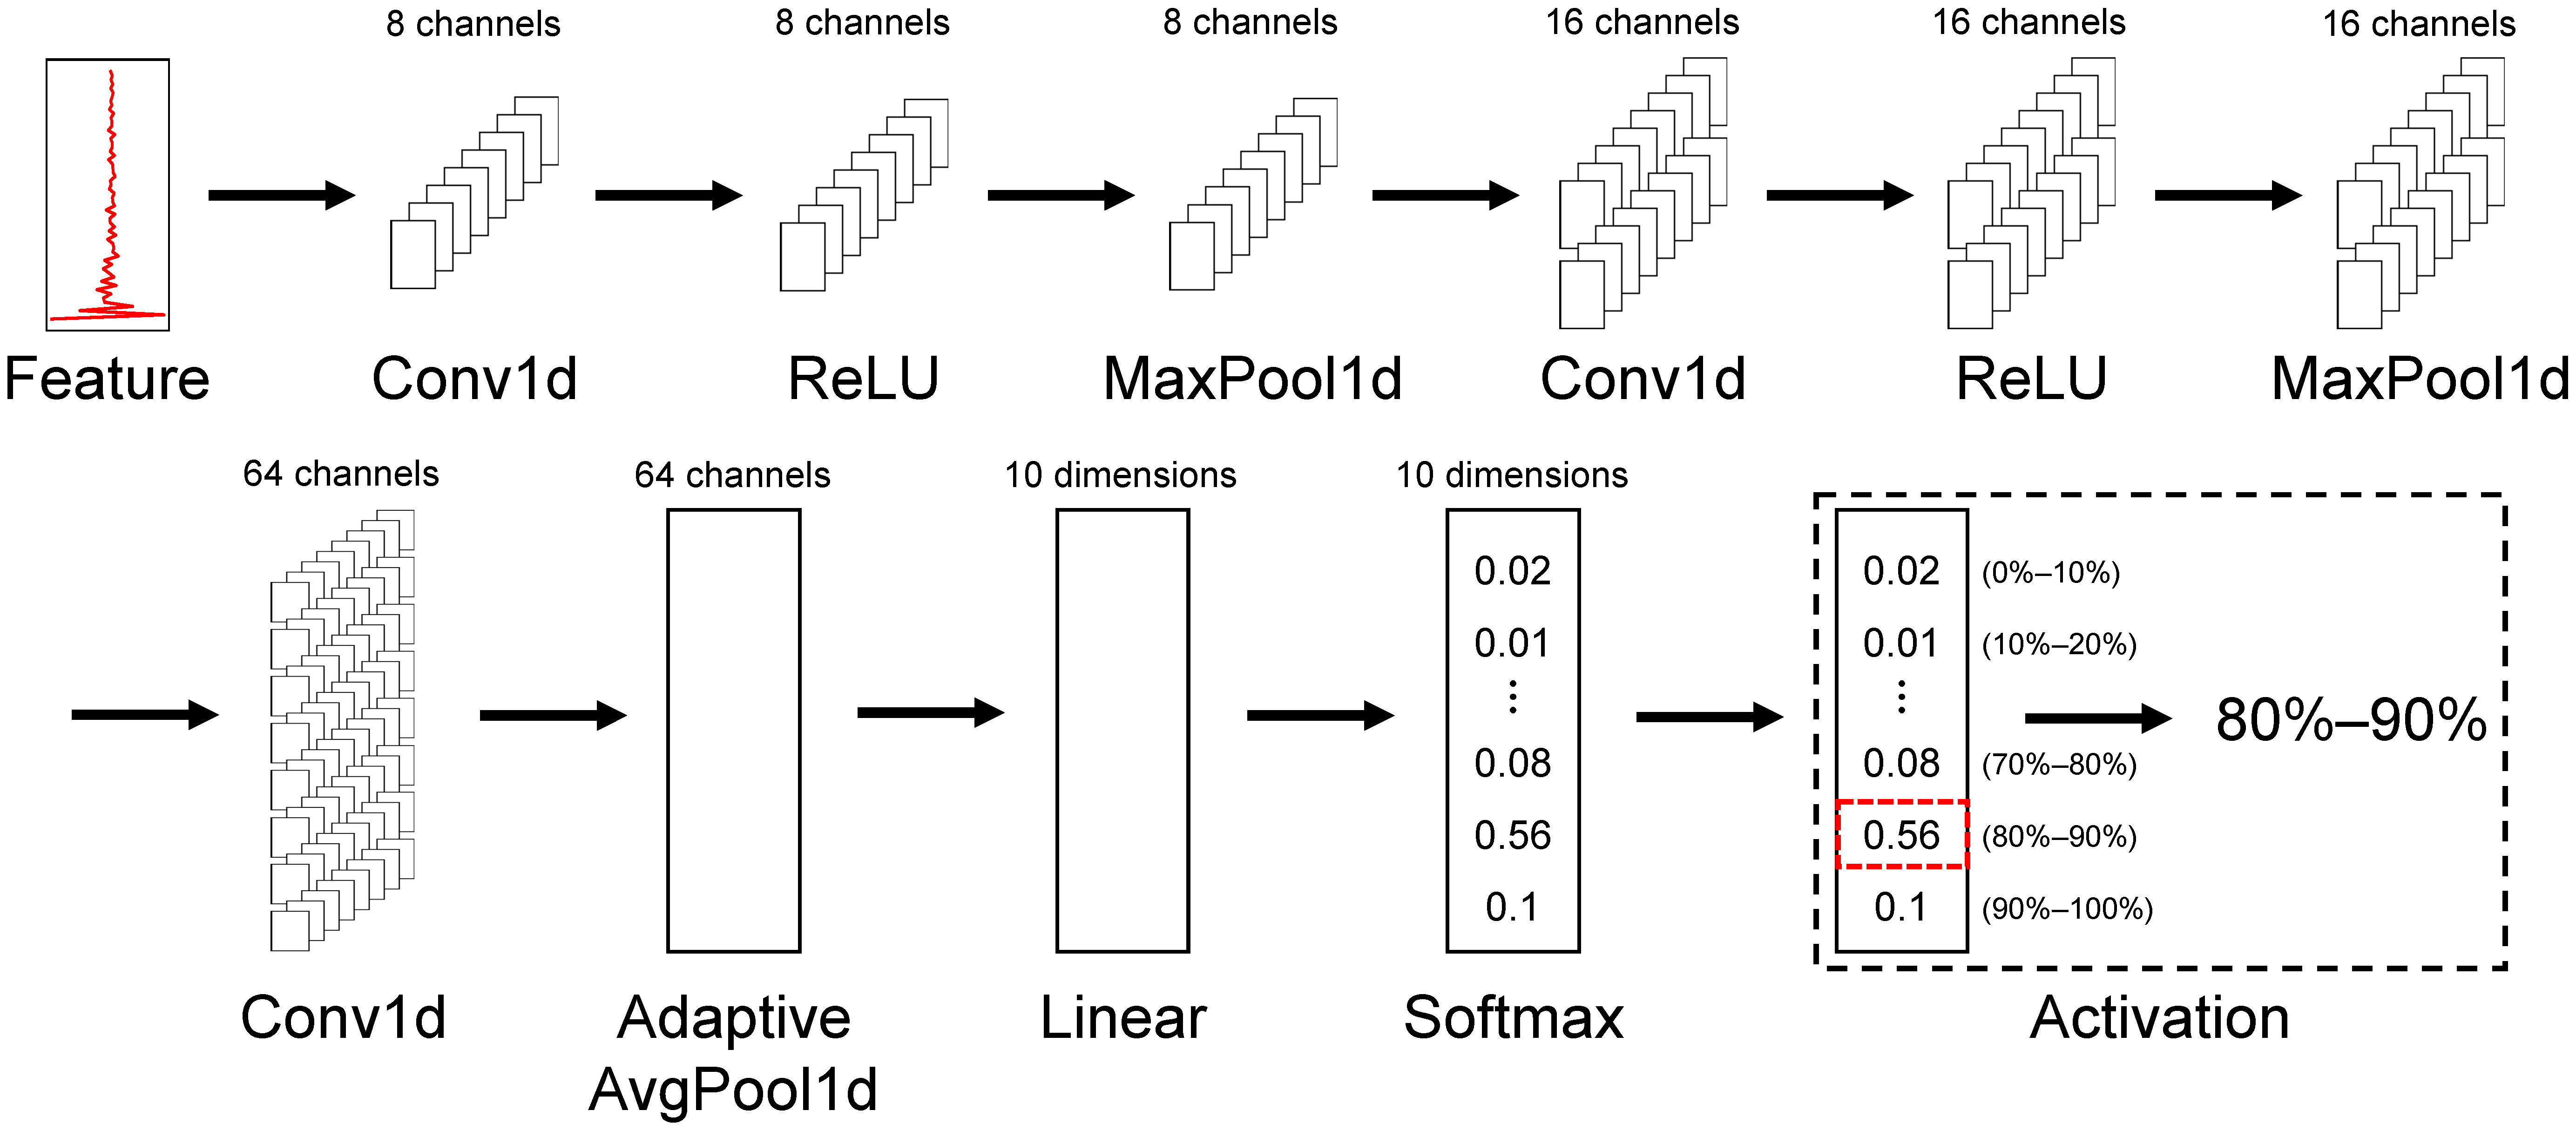
\includegraphics[width=0.8\linewidth]{figures/model.eps}
  \caption{Structure of estimation model.}
  \label{fig:model}
\end{figure}



% 4
\section{Evaluation}
\label{sec:evaluation}
We conducted an evaluation experiment to determine the effectiveness of the proposed method using previously collected pouring sounds.

% 4.1
\subsection{Data Collection}
The voice recorder app that comes with the Android smartphone (OPPO Find X3 Pro) was used to record pouring sounds, and data were collected in the following sequence. First, the faucet is opened to a certain degree and water flows. Next, we hold the smartphone in one hand and the bottle in the other. The bottle is placed close enough to the faucet that water can enter it, and the smartphone is placed near the bottle but not close enough to touch it. We pressed the Start Recording button on the app at the moment the bottle began to fill with water, and pressed the End Recording button at the moment the water overflowed. The pouring sound obtained in one recording process is considered to be one sample. \figref{data_acquisition} shows a photograph of the recording in progress. The data were collected from 20 samples using the five types of bottle shown in \figref{bottles} (100 samples in total) at a sampling frequency of 96 kHz while the faucet opening was kept constant. The bottles are, from left to right, an empty aluminum coffee can (Bottle A), an empty plastic dish detergent bottle (Bottle B), a plastic shampoo bottle (Bottle C), an empty plastic milk solution bottle (Bottle D), and a ceramic sake bottle (Bottle E), all of different shapes.

\begin{figure}[!t]
  \centering
  \includegraphics[width=0.8\linewidth]{figures/data_acquisition.eps}
  \caption{Collecting pouring sounds to be used in evaluation experiment.}
  \label{fig:data_acquisition}
\end{figure}

\begin{figure}[!t]
  \centering
  \includegraphics[width=0.8\linewidth]{figures/bottles.eps}
  \caption{Bottles used in evaluation experiment.}
  \label{fig:bottles}
\end{figure}


% 4.2
\subsection{Environment for Evaluation Experiments}
The collected pouring sounds are labeled in advance in accordance with the water level. The label $y[i]$ assigned to the $i$-th data, $x[i]$ $(i=0,\dots,L-1)$, of a pouring sound of length $L$ is obtained by the following equation.
\begin{equation}
  y[i]=i \times 100/(L-1)
\end{equation}

We performed segmentation using a sliding window with a window size of 0.2 seconds and a step width of 0.02 seconds. The labels are those assigned to the data at the end of the window.\par

The number of estimated classes was set to $C=[BOTTLES\_NUM,10,2]$, and respective estimation models were constructed. The number of output dimensions of the linear layer was changed to the number of estimated classes. When $C=BOTTLES\_NUM$ (5 in this paper), the model estimates the type of bottle into which water is being poured; for example, when $C=10$, it estimates the water level in the range of 0--100\% in increments of 10\%, and when $C=2$, we focus on whether or not the water overflows and the model estimates whether the water level is above 90\%. The batch size and number of epochs during the training phase of the estimation model were set to 100 and 1,000, respectively. The data used to train one epoch were extracted so that the bottle and water level labels were equally represented. Specifically, we extracted data equally from Bottle A (0\%--10\%), A (10\%--20\%), \dots, A (90\%--100\%), B (0\%--10\%), \dots, E (80\%--90\%), and E (90\%--100\%) when $C=[BOTTLES\_NUM,10]$ and from Bottle A (0\%--90\%), A (90\%--100\%), B (0\%--90\%), \dots, E (0\%--90\%), and E (90\%--100\%) when $C=2$. We did this because we segmented the data using a sliding window and thus needed to avoid bias in learning due to the presence of multiple data with the same label. We also created a bottle-independent estimation model for use in real environments, where none of the data from the bottles used for testing was used for training.


% 4.3
\subsection{Results and Discussion}

% 4.3.1
\subsubsection{Bottle Estimation Model}
For the model to estimate the type of bottle, 99 out of a total of 100 samples (20 samples $\times$ 5 bottles) of all bottles were used for training, and the estimation accuracy was tested on 50 segments extracted from the remaining one sample of data not used for training. The accuracy was calculated using the leave-one-session-out (LOSO) algorithm so that all 100 samples were test data. The average values of accuracy for each bottle are listed in \tabref{result_5}, where ``Average'' is the mean value of all accuracies. All results are rounded to the fourth decimal place. The confusion matrix, which sums all the estimation results, is shown in \figref{confusion_matrix_5}, and the evolution of the average loss for each bottle during the training phase is shown in \figref{loss}. The confusion matrix represents the number of actual labels input vertically and the number of estimated labels output horizontally.\par

The results showed that an average estimation accuracy of 0.642 was achieved. The high accuracy compared to the chance-level accuracy of 0.2 for the 5-class classification suggests that it is possible to estimate the type of bottle using the pouring sound. On the other hand, Bottle C had the worst accuracy of 0.559 in each bottle. We checked the confusion matrix and found that data actually belonging to Bottle A was mistakenly estimated as belonging to Bottle C. This indicates that the pouring sounds of Bottle A and Bottle C may have been similar, possibly due to their similar shape and caliber size.

\begin{table}[!t]
  \small
  \centering
  \caption{Accuracy results of bottle estimation model. ($C=BOTTLES\_NUM$)}
  \begin{tabular}{c|c} \hline\hline
    Bottle & Accuracy \\ \hline
    A & 0.587 \\
    B & 0.643 \\
    C & 0.559 \\
    D & 0.666 \\
    E & 0.755 \\ \hline
    Average & 0.642 \\ \hline
  \end{tabular}
  \label{tab:result_5}
\end{table}

\begin{figure}[!t]
  \centering
  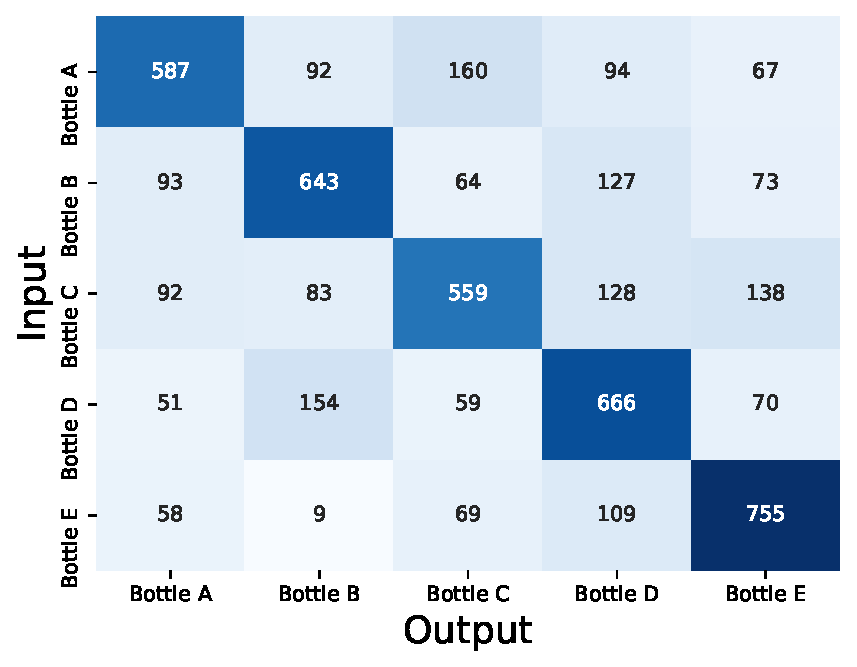
\includegraphics[width=0.4\linewidth]{figures/confusion_matrix_5.eps}
  \caption{Confusion matrix in bottle estimation.}
  \label{fig:confusion_matrix_5}
\end{figure}

\begin{figure}[!t]
  \centering
  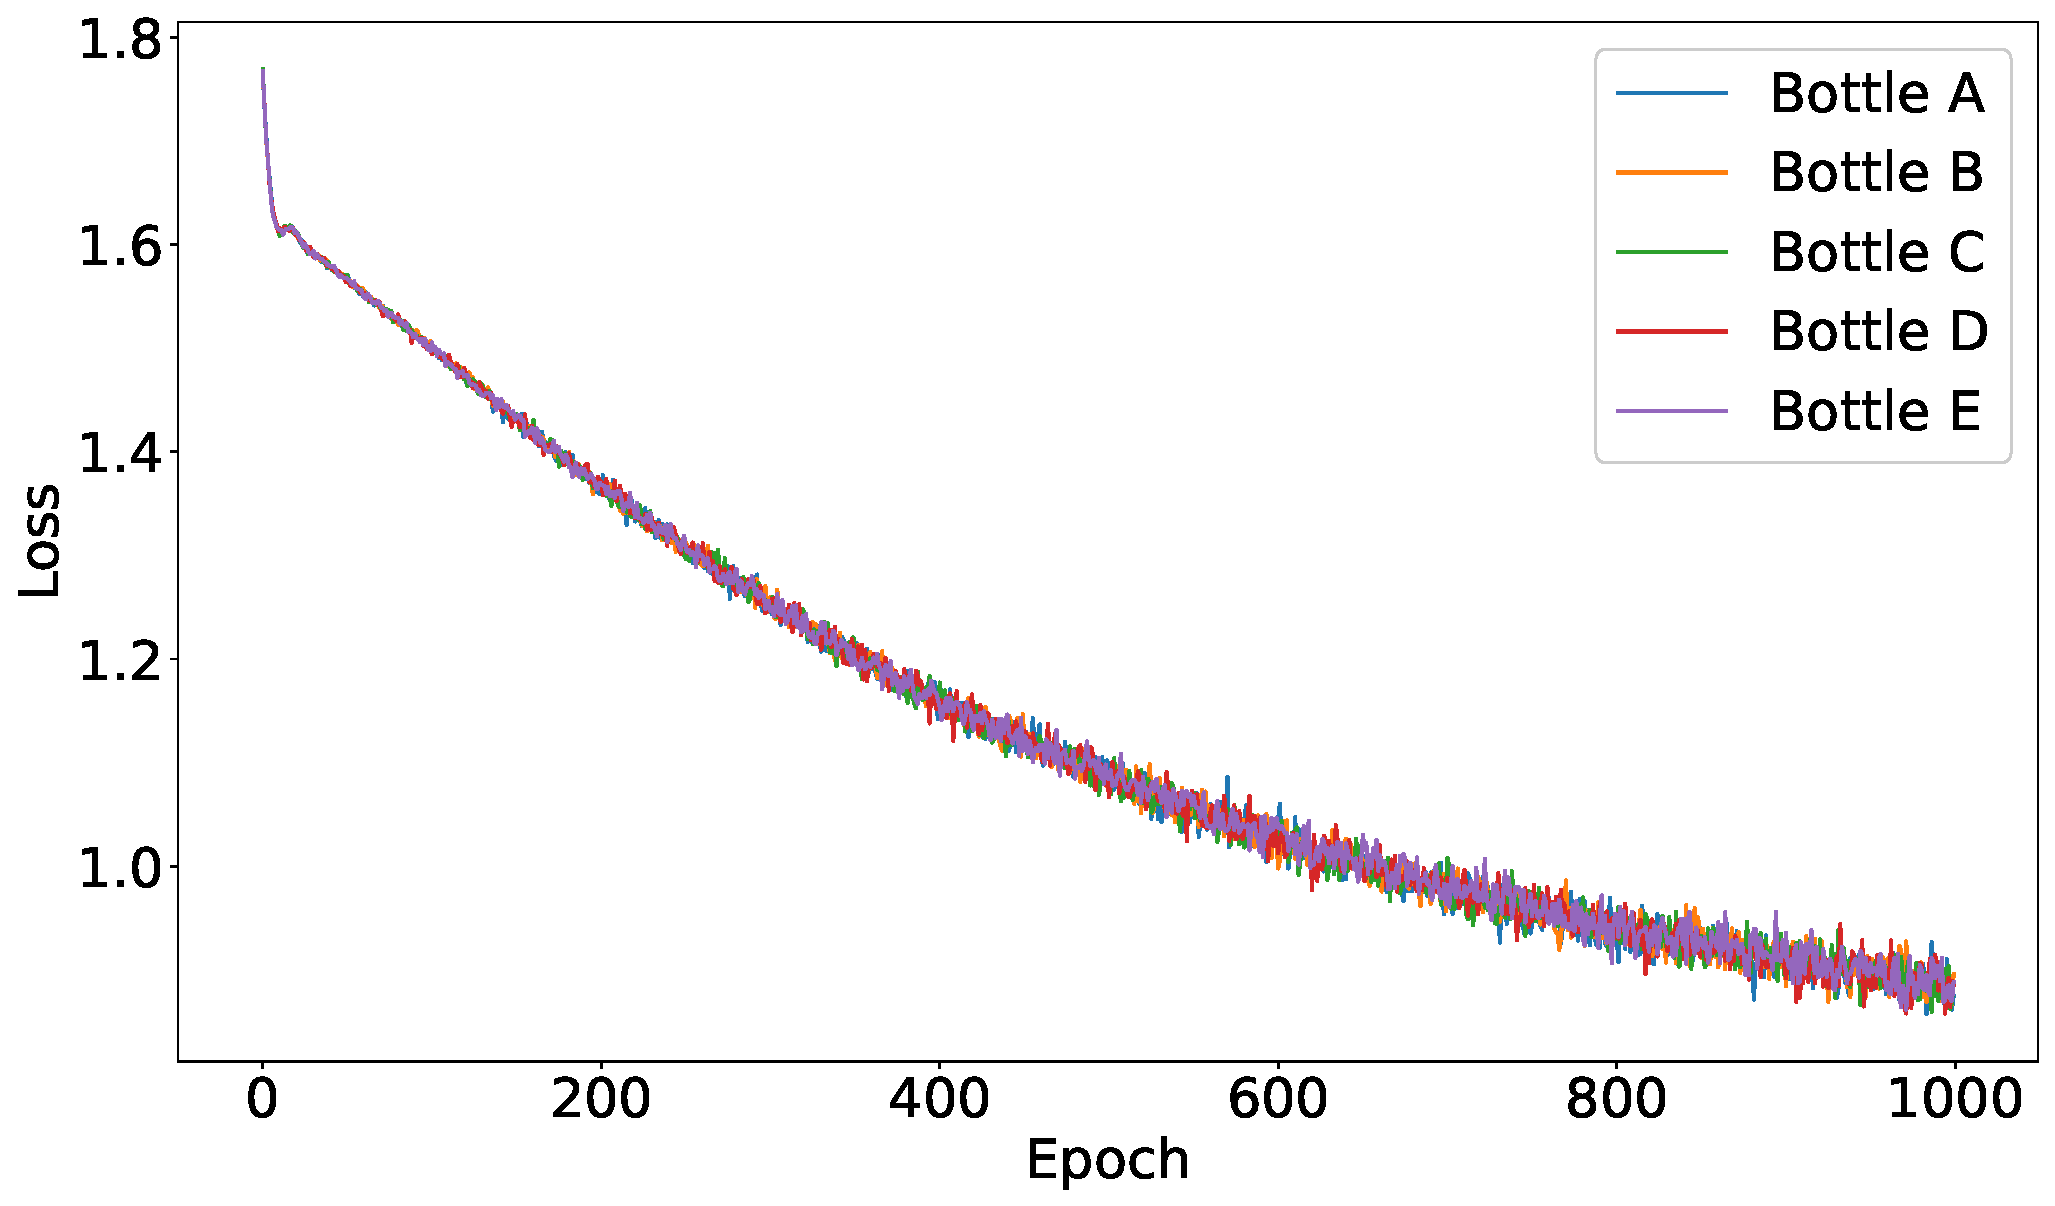
\includegraphics[width=0.8\linewidth]{figures/loss_5.eps}
  \caption{Change in loss during training phase of bottle estimation model.}
  \label{fig:loss}
\end{figure}

% 4.3.2
\subsubsection{Water Level Estimation Model}
For a model that estimates water levels in the range of 0--100\% in 10\% increments, 99 out of a total of 100 samples (20 samples $\times$ 5 bottles) of all bottles were used for training, and the estimation accuracy of the bottle-dependent estimation model was tested on 50 segments extracted from the remaining one sample of data not used for training. The accuracy was calculated using the LOSO algorithm so that all 100 samples were test data. The average values of accuracy for each bottle are listed in \tabref{result_10_dependent}, and the confusion matrix summing all the estimation results is shown in \figref{confusion_matrix_10_dependent}. Test data were extracted so that all ten classes of labels appeared uniformly.\par

A total of 80 samples (20 samples $\times$ 4 bottles) from four bottles were used for training, and the estimation accuracy of the bottle-independent estimation model was tested on 500 segments extracted from 20 samples of data from the one remaining bottle not used for training. The accuracy was calculated using the leave-one-bottle-out (LOBO) algorithm so that all data for five bottles were test data. The average values of accuracy for each bottle are listed in \tabref{result_10_independent}, and the confusion matrix summing all the estimation results is shown in \figref{confusion_matrix_10_independent}. Test data were extracted so that all ten classes of labels appeared uniformly.\par

The results show an average accuracy of 0.462 for the bottle-dependent estimation model and 0.308 for the bottle-independent estimation model. In the results for each bottle, Bottle B had the worst accuracy for both the bottle-dependent and the bottle-independent estimation models. Bottle B had the largest volume, resulting in a longer pour sound and more segments extracted from each sample, so it is possible that the features were not as trained as in the other bottles, even though they had the same number of epochs. However, this is a high accuracy compared to 0.1, which is the chance-level accuracy for 10-class classification. While we feel it is feasible to estimate the water level using the pouring sound, the accuracy needs to be improved for use in real environments. In terms of the confusion matrix of the bottle-dependent estimation model, the accuracy could possibly be improved by expanding the estimated water level from 10\% increments, since there are many cases of mis-estimation for labels with similar water levels. Since the estimation accuracy of the bottle-dependent estimation model is approximately 0.15 higher than that of the bottle-independent estimation model, the accuracy could be significantly improved by building an estimation model for each bottle of similar shape and implementing a mechanism such as switching the model to be used before estimation.

\begin{table}[!t]
  \small
  \centering
  \caption{Accuracy results of water level estimation model. ($C=10$)}
  \begin{minipage}[t]{0.45\linewidth}
    \centering
    \subcaption{Bottle-dependent estimation model.}
    \begin{tabular}{c|c} \hline\hline
    Bottle & Accuracy \\ \hline
    A & 0.553 \\
    B & 0.333 \\
    C & 0.479 \\
    D & 0.424 \\
    E & 0.519 \\ \hline
    Average & 0.462 \\ \hline
    \end{tabular}
    \label{tab:result_10_dependent}
  \end{minipage}
  \begin{minipage}[t]{0.45\linewidth}
    \centering
    \subcaption{Bottle-independent estimation model.}
    \begin{tabular}{c|c} \hline\hline
    Bottle & Accuracy \\ \hline
    A & 0.436 \\
    B & 0.198 \\
    C & 0.374 \\
    D & 0.290 \\
    E & 0.244 \\ \hline
    Average & 0.308 \\ \hline
    \end{tabular}
    \label{tab:result_10_independent}
  \end{minipage}
  \label{tab:result_10}
\end{table}

\begin{figure}[!t]
  \centering
  \begin{minipage}[t]{0.45\linewidth}
    \centering
    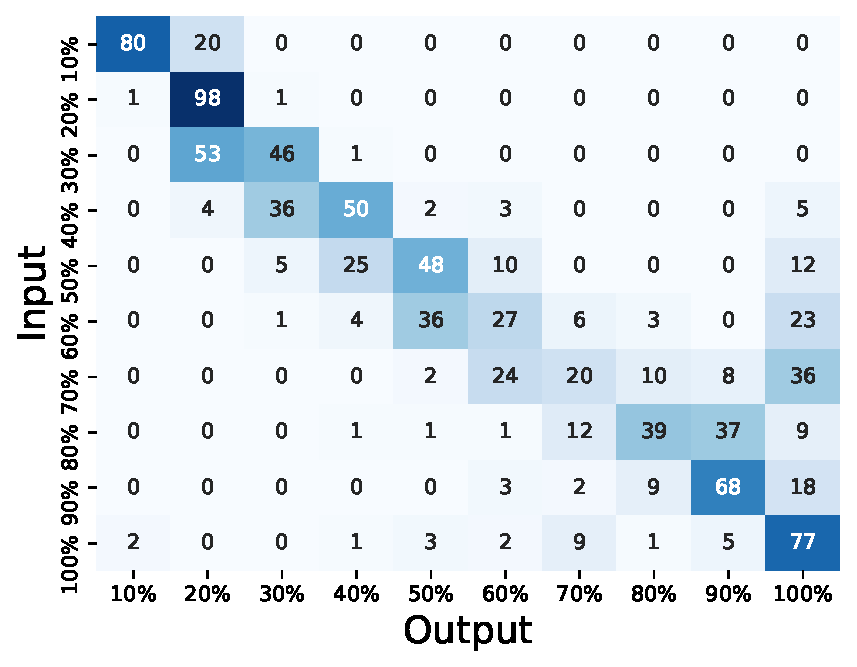
\includegraphics[width=0.9\linewidth]{figures/confusion_matrix_10_dependent_coffee.eps}
    \subcaption{Bottle A}
  \end{minipage}
  \begin{minipage}[t]{0.45\linewidth}
    \centering
    \includegraphics[width=0.9\linewidth]{figures/confusion_matrix_10_dependent_dishwashing.eps}
    \subcaption{Bottle B}
  \end{minipage}
  \begin{minipage}[t]{0.45\linewidth}
    \centering
    \includegraphics[width=0.9\linewidth]{figures/confusion_matrix_10_dependent_shampoo.eps}
    \subcaption{Bottle C}
  \end{minipage}
  \begin{minipage}[t]{0.45\linewidth}
    \centering
    \includegraphics[width=0.9\linewidth]{figures/confusion_matrix_10_dependent_skinmilk.eps}
    \subcaption{Bottle D}
  \end{minipage}
  \begin{minipage}[t]{0.45\linewidth}
    \centering
    \includegraphics[width=0.9\linewidth]{figures/confusion_matrix_10_dependent_tokkuri.eps}
    \subcaption{Bottle E}
  \end{minipage}
  \caption{Confusion matrix in water level estimation (bottle-dependent estimation model).}
  \label{fig:confusion_matrix_10_dependent}
\end{figure}

\begin{figure}[!t]
  \centering
  \begin{minipage}[t]{0.45\linewidth}
    \centering
    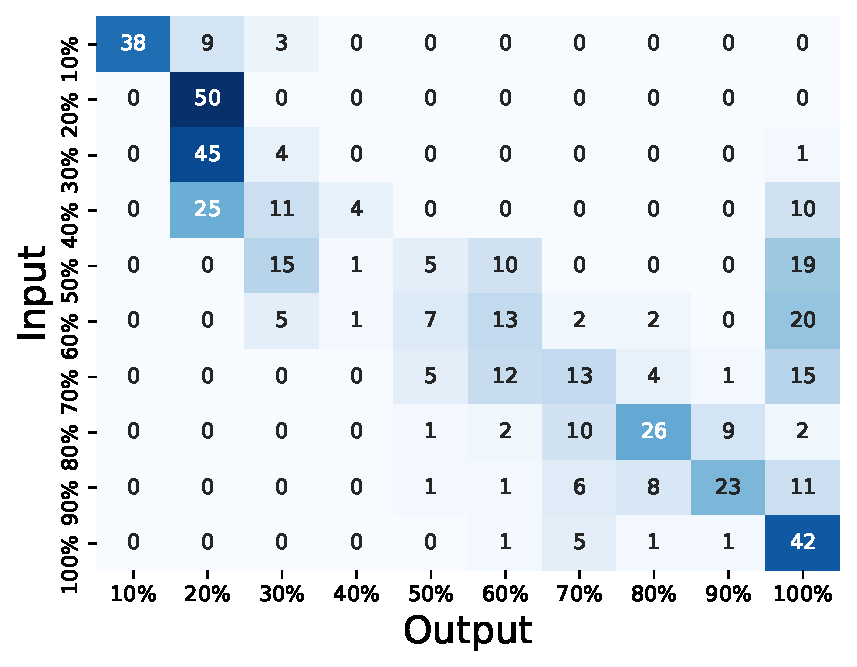
\includegraphics[width=0.9\linewidth]{figures/confusion_matrix_10_independent_coffee.eps}
    \subcaption{Bottle A}
  \end{minipage}
  \begin{minipage}[t]{0.45\linewidth}
    \centering
    \includegraphics[width=0.9\linewidth]{figures/confusion_matrix_10_independent_dishwashing.eps}
    \subcaption{Bottle B}
  \end{minipage}
  \begin{minipage}[t]{0.45\linewidth}
    \centering
    \includegraphics[width=0.9\linewidth]{figures/confusion_matrix_10_independent_shampoo.eps}
    \subcaption{Bottle C}
  \end{minipage}
  \begin{minipage}[t]{0.45\linewidth}
    \centering
    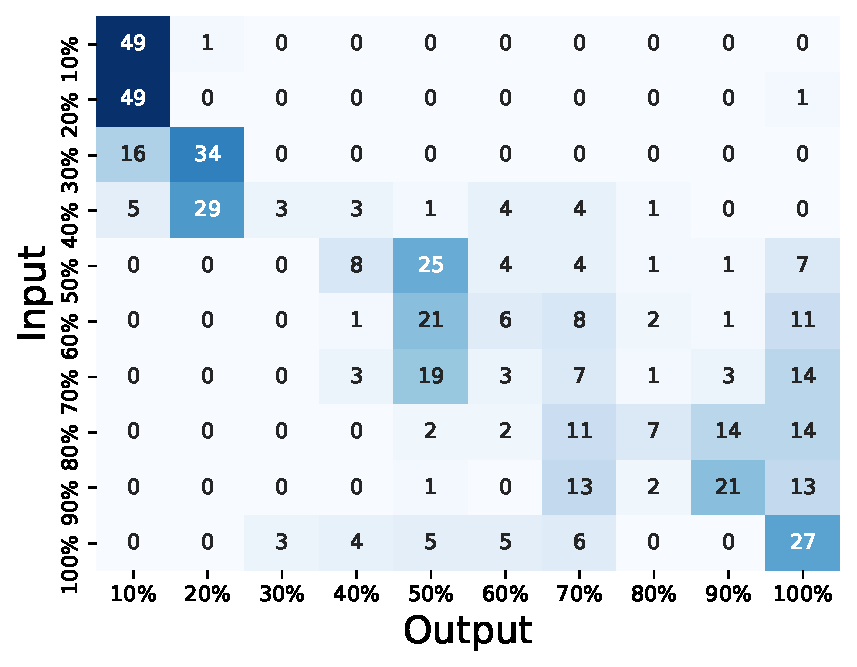
\includegraphics[width=0.9\linewidth]{figures/confusion_matrix_10_independent_skinmilk.eps}
    \subcaption{Bottle D}
  \end{minipage}
  \begin{minipage}[t]{0.45\linewidth}
    \centering
    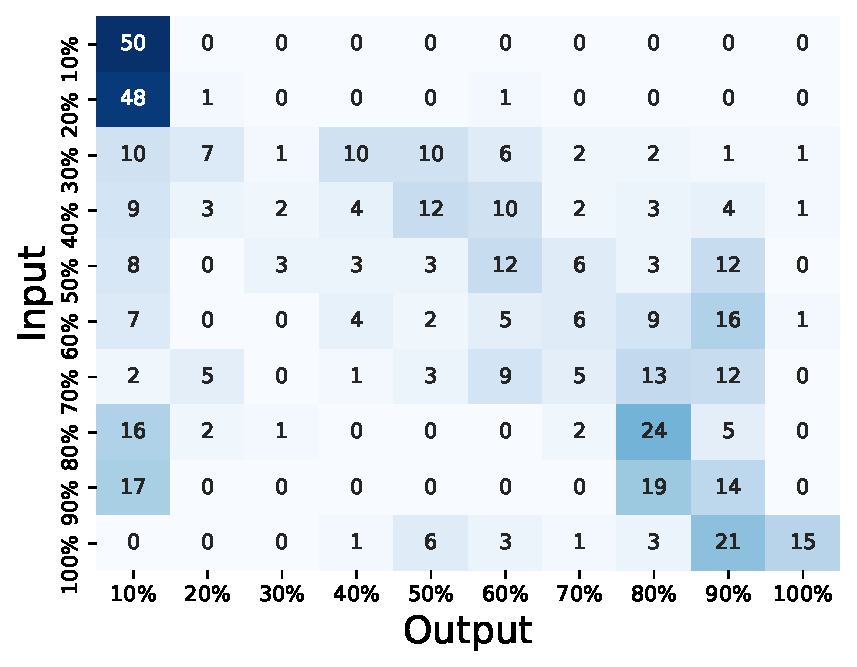
\includegraphics[width=0.9\linewidth]{figures/confusion_matrix_10_independent_tokkuri.eps}
    \subcaption{Bottle E}
  \end{minipage}
  \caption{Confusion matrix in water level estimation (bottle-independent estimation model).}
  \label{fig:confusion_matrix_10_independent}
\end{figure}

% 4.3.3
\subsubsection{Overflow Detection Model}
For a model that estimates whether the water level is above 90\% by focusing on whether the water overflows or not, 99 out of a total of 100 samples (20 samples $\times$ 5 bottles) of all bottles were used for training, and the estimation accuracy of the bottle-dependent estimation model was tested on 30 segments extracted from the remaining one sample of data not used for training. The accuracy was calculated using the LOSO algorithm so that all 100 samples were test data. The average accuracy values for each bottle are listed in \tabref{result_2_dependent}. The test data were extracted so that the two classes to be estimated (0\%--90\% and 90\%--100\%) appeared uniformly.\par

A total of 80 samples (20 samples $\times$ 4 bottles) from four bottles were used for training, and the estimation accuracy of the bottle-independent estimation model was tested on 500 segments extracted from 20 samples of data from the one remaining bottle not used for training. The accuracy was calculated using the LOBO algorithm so that all data for five bottles were test data. The average accuracy values for each bottle are listed in \tabref{result_2_independent}. The test data were extracted so that the two classes (0\%--90\% and 90\%--100\%) to be estimated appeared uniformly.\par

The results showed that the bottle-dependent and bottle-independent estimation models achieved an average accuracy of 0.83 and 0.744, indicating that it is possible to detect the overflow just before it occurs regardless of which bottle is used. The high accuracy of the overflow detection suggests that it can be implemented in a faucet-mounted device. Further improvement in accuracy can be expected by expanding the range of water estimation level from 0\%--90\% and 90\%--100\% to 0\%--80\% and 80\%--100\%.

\begin{table}[!t]
  \small
  \centering
  \caption{Accuracy results of overflow detection model. ($C=2$)}
  \begin{minipage}[t]{0.45\linewidth}
    \centering
    \subcaption{Bottle-dependent estimation model.}
    \begin{tabular}{c|c} \hline\hline
    Bottle & Accuracy \\ \hline
    A & 0.852 \\
    B & 0.755 \\
    C & 0.782 \\
    D & 0.878 \\
    E & 0.882 \\ \hline
    Average & 0.830 \\ \hline
    \end{tabular}
    \label{tab:result_2_dependent}
  \end{minipage}
  \begin{minipage}[t]{0.45\linewidth}
    \centering
    \subcaption{Bottle-independent estimation model.}
    \begin{tabular}{c|c} \hline\hline
    Bottle & Accuracy \\ \hline
    A & 0.760 \\
    B & 0.668 \\
    C & 0.770 \\
    D & 0.770 \\
    E & 0.750 \\ \hline
    Average & 0.744 \\ \hline
    \end{tabular}
    \label{tab:result_2_independent}
  \end{minipage}
  \label{tab:result_2}
\end{table}



% 5
\section{Future Work}
\label{sec:future_work}
The evaluation experiments demonstrate that high estimation accuracy can be obtained when the overflow detection model is used, regardless of which bottle is used. However, the water level estimation model had an average accuracy of only 0.462, even in the bottle-dependent estimation model. In the future, we plan to improve the accuracy by building a water level estimation model for each bottle and switching which model is used in accordance with the results obtained from the bottle estimation model, and to develop a method in which a majority decision is made on the basis of the estimation results of five consecutive windows. We will also implement a faucet-mounted device incorporating the proposed method and evaluate its effectiveness.



% 6
\section{Conclusion}
\label{sec:conclution}
In this paper, we proposed a method to estimate the water level in a container by acquiring the sound of water pouring, assuming a device attached to a faucet, so that the water level can be correctly determined even in a container whose internal conditions are difficult to grasp. We implemented several estimation models and conducted experiments to evaluate the estimation accuracy using five bottles. The results showed that the bottle estimation model had an average accuracy of 0.642, the water level estimation model had respective averages of 0.462 and 0.308 for the bottle-dependent and bottle-independent models, and the overflow detection model had respective averages of 0.83 and 0.744 for the bottle-dependent and bottle-independent models. These results indicate that, while the accuracy of the water level estimation needs to be improved, the overflow detection can be achieved regardless of the container type and may be used in real environments. In the future, we plan to improve the model for better estimation accuracy and to implement a faucet-mounted device that incorporates a function to stop water injection just before it becomes full.

%%
%% The acknowledgments section is defined using the "acks" environment
%% (and NOT an unnumbered section). This ensures the proper
%% identification of the section in the article metadata, and the
%% consistent spelling of the heading.
% \begin{acks}
% To Robert, for the bagels and explaining CMYK and color spaces.
% \end{acks}

%%
%% The next two lines define the bibliography style to be used, and
%% the bibliography file.
\bibliographystyle{ACM-Reference-Format}
\bibliography{references}

%%
%% If your work has an appendix, this is the place to put it.
% \appendix

% \section{Research Methods}

% \subsection{Part One}

% Lorem ipsum dolor sit amet, consectetur adipiscing elit. Morbi
% malesuada, quam in pulvinar varius, metus nunc fermentum urna, id
% sollicitudin purus odio sit amet enim. Aliquam ullamcorper eu ipsum
% vel mollis. Curabitur quis dictum nisl. Phasellus vel semper risus, et
% lacinia dolor. Integer ultricies commodo sem nec semper.

% \subsection{Part Two}

% Etiam commodo feugiat nisl pulvinar pellentesque. Etiam auctor sodales
% ligula, non varius nibh pulvinar semper. Suspendisse nec lectus non
% ipsum convallis congue hendrerit vitae sapien. Donec at laoreet
% eros. Vivamus non purus placerat, scelerisque diam eu, cursus
% ante. Etiam aliquam tortor auctor efficitur mattis.

% \section{Online Resources}

% Nam id fermentum dui. Suspendisse sagittis tortor a nulla mollis, in
% pulvinar ex pretium. Sed interdum orci quis metus euismod, et sagittis
% enim maximus. Vestibulum gravida massa ut felis suscipit
% congue. Quisque mattis elit a risus ultrices commodo venenatis eget
% dui. Etiam sagittis eleifend elementum.

% Nam interdum magna at lectus dignissim, ac dignissim lorem
% rhoncus. Maecenas eu arcu ac neque placerat aliquam. Nunc pulvinar
% massa et mattis lacinia.

\end{document}
\endinput
%%
%% End of file `sample-authordraft.tex'.
